% Chapter Template

\chapter{Software requirement specification} % Main chapter title

\label{ChapterX} % Change X to a consecutive number; for referencing this chapter elsewhere, use \ref{ChapterX}

\lhead{ \emph{Software requirement specification}} % Change X to a consecutive number; this is for the header on each page - perhaps a shortened title

%----------------------------------------------------------------------------------------
%	SECTION 1
%----------------------------------------------------------------------------------------

\section{Introduction}



\subsection{Purpose}

The software requirement specification should provide all needed information to develop the context extraction framework and define all delivery objects. All interfaces to external components, input and output data, deployment considerations and quality attribute should be well defined within this document.


\subsection{Scope}


The context extraction framework will perform automated text extraction on a set of HTML test data with two to three different text extraction algorithms. The performance of each algorithm is measured and an output file with the measured results is generated.

%----------------------------------------------------------------------------------------
%	SECTION 2
%----------------------------------------------------------------------------------------

\section{General description}

\subsection{Operating Environment}

\subsubsection{Local environment}

\begin{tabular}{| p{3cm} | p{3cm} |}
	\hline
	JDK & 1.7.X  \\ \hline
	Gradle & 1.1 \\ \hline
	Eclipse Keppler & 2.X \\ \hline
	git & 1.9.X \\ \hline
	python & 2.7.X \\ \hline
\end{tabular}


\subsubsection{Continuous Integration Environment}

\begin{tabular}{| p{3cm} | p{3cm} |}
	\hline
	Open JDK & 1.6.X  \\ \hline
	Open JDK & 1.7.X  \\ \hline
	Oracle JDK & 1.7.X \\ \hline
	Oracle JDK & 1.8.X  \\ \hline
	Gradle & 1.1 \\ \hline
	Travis CI &  \\ \hline
\end{tabular}



\subsection{Design and Implementation Constraints}

\subsubsection{User interface}
As parts of the text extraction framework may be implemented in a server environment and a user interface is not desired from the client so there will be no graphical user interface. The application is built, deployed and started by gradle. While the application is running, no interaction with the user is needed.


\section{System Features}

This section specifies all system features. Each feature is specified more close with multiple user stories but all important information such as external dependencies and output files are defined in this chapter. The related user stories are located in the planning section.  



\begin{landscape}

\subsection{Basic functionality}
Following diagram and text describes the basic functionality of the application.

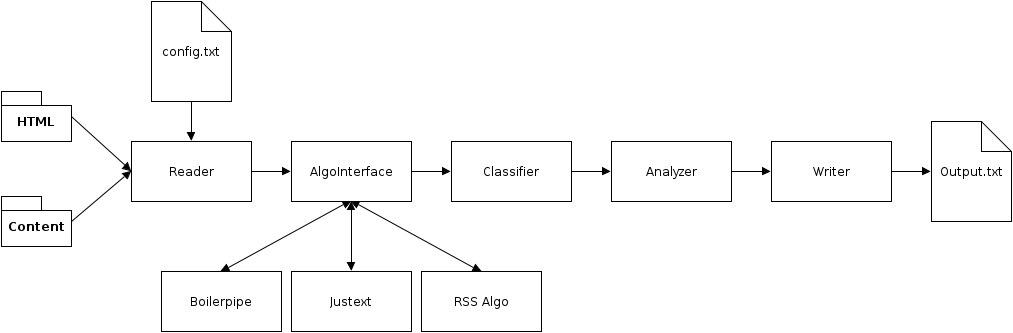
\includegraphics[width=24cm]{Pictures/Sysspec.png}

There are two folders defined by a configuration flies which. The HTML folder contains plain HTML files of web pages. The content folder contains text files with the relevant content of the related HTML files. As soon as a test is started the HTML file and the text file are read and the HTML file is extracted and classified with all the available algorithms. The result of the classification is then compared to the text file with the relevant content and performance data is generated. This performance data is then analyzed with statistical methods. 

\end{landscape}



\subsection{Overview}

	\begin{tabular}{ | p{1cm} | p{9cm} |p{3cm} |}
	\hline
	\textbf{ID}	& \textbf{Name}   					& \textbf{Relevance}	\\ \hline
	f1  		& Read configuration  								& needed 				\\ \hline
	f2  		& Create test										& needed 				\\ \hline
	f3  		& Integration Justext algorithm  					& needed 				\\ \hline
	f4  		& Integration Boilerpipe algorithm  				& needed 				\\ \hline
	f5  		& Evaluation and Implementation RSS feed algorithm 	& nice to have			\\ \hline
	f6  		& Evaluation of Classification Text					& needed 				\\ \hline
	f7  		& Evaluation of Classification Block	  			& nice to have			\\ \hline
	f8  		& Analyze Data 										& needed 				\\ \hline
	\end{tabular} \\



\subsubsection{Read configuration}

	\begin{tabular}{ | p{3cm} | p{12cm} |}
	\hline
	\textbf{Name} 				& Read configuration 				\\ \hline
	\textbf{Feature id} 		& f1 				\\ \hline
	\textbf{Description} 		& The text extraction framework is configurable with an external text file. The configuration file will contain following items:
							        \begin{itemize}
							        \item Path to folder with HTML files
							        \item Path to folder with text files
							        \item Path to folder with output files
							        \item Configuration for algorithms
							        \item etc.
						        \end{itemize} 
						        The configuration file location is defined as a relative path to the source directory and structured in a key value list: 

						        \lstinputlisting{Code/config_template.txt} \\ \hline
	\textbf{Relevance} 			& needed 			\\ \hline
	\textbf{Related stories} 	& tbd		\\ \hline
	\end{tabular} \\

\subsubsection{Create test}


	\begin{tabular}{ | p{3cm} | p{12cm} |}
	\hline
	\textbf{Name} 				& Create test \\ \hline
	\textbf{Feature id} 		& f2 \\ \hline
	\textbf{Description} 		& A test contains two input files which are a HTML file and a text file. They are located in the directories defined by the configuration. As soon as the test framework finds an HTML and a text file with the same name, a new test is created, the files are read and the test is started.\\ \hline
	\textbf{Relevance} 			& needed \\ \hline
	\textbf{Related stories} 	& tbd \\ \hline
	\end{tabular} \\

\subsubsection{Integration Justext algorithm}


	\begin{tabular}{ | p{3cm} | p{12cm} |}
	\hline
	\textbf{Name} 				& Integration Justext algorithm \\ \hline
	\textbf{Feature id} 		& f3 \\ \hline
	\textbf{Description} 		& Justext is implemented in python so a service is needed to call the python script and get the extracted text or the extracted blocks.\\ \hline
	\textbf{Relevance} 			& needed \\ \hline
	\textbf{Related stories} 	& tbd \\ \hline
	\end{tabular} \\

\subsubsection{Integrate Boilerpipe algorithm}

	\begin{tabular}{ | p{3cm} | p{12cm} |}
	\hline
	\textbf{Name} 				& Integration Boilerpipe algorithm \\ \hline
	\textbf{Feature id} 		& f4 \\ \hline
	\textbf{Description} 		& Boilerplate is implemented in Java so an interface is needed to call the Boilerplate component and get the extracted text or the extracted blocks.\\ \hline
	\textbf{Relevance} 			& needed \\ \hline
	\textbf{Related stories} 	& tbd \\ \hline
	\end{tabular} \\

\subsubsection{Integrate RSS feed algorithm}

\begin{tabular}{ | p{3cm} | p{12cm} |}
	\hline
	\textbf{Name} 				& Evaluation and implementation RSS feed algorithm \\ \hline
	\textbf{Feature id} 		& f5 \\ \hline
	\textbf{Description} 		& The basic idea of the RSS feed algorithm is to match the content of a HTML document with the related RSS feed and define the relevant content like that. This need to be evaluated, implemented and integrated into the text extraction framework  \\ \hline
	\textbf{Relevance} 			& nice to have\\ \hline
	\textbf{Related stories} 	& tbd \\ \hline
	\end{tabular} \\

\subsubsection{Evaluation of classification text}

	\begin{tabular}{ | p{3cm} | p{12cm} |}
	\hline
	\textbf{Name} 				& Evaluation of classification \\ \hline
	\textbf{Feature id} 		& f6 \\ \hline
	\textbf{Description} 		& All the text extraction algorithms return an extracted document as text. This document needs to be checked for correctness. To do so the result from the algorithms is compared with the predefined content. This evaluation and classification is defined in more detail here: \ref{subsec:Further explanation for evaluation of classification}
								\begin{itemize}
							        \item Check each classified block from the algorithms if it's content can be found in the content file
							        \item Categorize all blocks as true negative and false positive
							        \item Put the results into an output text file (structure output file: tbd)
						        \end{itemize} \\ \hline
	\textbf{Relevance} 			& needed\\ \hline
	\textbf{Related stories} 	& tbd \\ \hline
	\end{tabular} \\


\subsubsection{Evaluation of classification blocks}

	\begin{tabular}{ | p{3cm} | p{12cm} |}
	\hline
	\textbf{Name} 				& Evaluation of classification blocks \\ \hline
	\textbf{Feature id} 		& f6 \\ \hline
	\textbf{Description} 		& A more detailed evaluation of the algorithms could be done if not only the text is classified but each block of an HTML file. To do so, the implementation of Justext and Boilerpipe have to be addapted that they return classified blocks instead of the extracted text. These blocks are then compared with the predefined content and classified. This evaluation and classification is defined in more detail in following section: \ref{subsec:Further explanation for evaluation of classification}
								\begin{itemize}
							        \item Check each classified block from the algorithms if it's content can be found in the content file
							        \item Categorize all blocks as true negative and false positive
							        \item Put the results into an output text file (structure output file: tbd)
						        \end{itemize} \\ \hline
	\textbf{Relevance} 			& nice to have\\ \hline
	\textbf{Related stories} 	& tbd \\ \hline
	\end{tabular} \\





\subsubsection{Analyze data}

	\begin{tabular}{ | p{3cm} | p{12cm} |}
	\hline
	\textbf{Name} 				& Analyze data \\ \hline
	\textbf{Feature id} 		& f7 \\ \hline
	\textbf{Description} 		&  From the results of the comparison several further values can be evaluated for a better understanding of the results. These values are described in more detail in following section: \ref{subsec:Further explanation for evaluation of classification}
								    \\ \hline
	\textbf{Relevance} 			& needed \\ \hline
	\textbf{Related stories} 	& tbd \\ \hline
	\end{tabular} \\

%    \item Presicion: $\frac{TP}{TP + FP}$
%    \item Recall/True positive rate (TPR): $\frac{TP}{TP + FN}$
%    \item false positive rate (FPR: $\frac{FP}{FP + TN}$
%    \item F-measure: $2* \frac{presicion * recall}{presicion + recall}$
%    \item Reciever Operation Characteristics (ROC): $TPR = f(FPR)$

	\begin{tabular}{ | p{3cm} | p{12cm} |}
	\hline
	\textbf{Name} 				& Visualize data \\ \hline
	\textbf{Feature id} 		& f8 \\ \hline
	\textbf{Description} 		& The calculated values from feature f8 are visualized in diagrams. (tbd: which tool)\\ \hline
	\textbf{Relevance} 			& tbd\\ \hline
	\textbf{Related stories} 	& tbd \\ \hline
	\end{tabular} \\


\subsection{Further explanation for evaluation of classification}
\label{subsec:Further explanation for evaluation of classification}


The general meaning of the expressions true positive, true negative, false positive and false negative related to the text extraction topic is shown in following table:

\begin{table}[h]
\begin{tabular}{|p{4cm} |p{5cm} |p{5cm} |}\hline
          								& \textbf{Classified as content} 	& \textbf{Classified as boilerplate} 	\\ \hline
\textbf{Acutal content} 				& True positive (TP)				& True negative (TN)					\\ \hline
\textbf{Actual boilerplate} 			& True negative (TN)       			& False negative (FN)				 	\\ \hline
\end{tabular}
\end{table}


\subsubsection{Evaluation the results as text}

When the results are compared based on the text, the expressions are interpreted as follow:

 \begin{table}[h]
\begin{tabular}{|p{4cm} |p{5cm} |p{5cm} |}
\hline         								& \textbf{Classified as content} 							& \textbf{Classified as boilerplate} 	\\ \hline
\textbf{Acutal content} 				& Number of words classified as content and are content		& Number of words classified as content but are boilerplate			\\ \hline
\textbf{Actual boilerplate} 			& Number of words classified as content but are boilerplate & Number of words classified as boilerplate and are boilerplate	 	\\ \hline
\end{tabular}
\end{table}

\subsubsection{Evaluation the results as blocks}

When the results are compared based on HTML blocks, the expressions are interpreted as follow:

When the results are compared based on the text the expressions are interpreted as follow:

 \begin{table}[h]
\begin{tabular}{|p{4cm} |p{5cm} |p{5cm} |}
\hline         								& \textbf{Classified as content} 								& \textbf{Classified as boilerplate} 								\\ \hline
\textbf{Acutal content} 				& Number of blocks classified as content and are content		& Number of blocks classified as content but are boilerplate		\\ \hline
\textbf{Actual boilerplate} 			& Number of blocks classified as content but are boilerplate 	& Number of blocks classified as boilerplate and are boilerplate	\\ \hline
\end{tabular}
\end{table}

\subsubsection{Analytical values}

The results of the comparison deliver basic characteristics which can be used to calculate statistical values which help to analyze the test outcome.
										
\textbf{Recall / Sensitivity /True positive rate / TPR }

Recall is the probability that a relevant document is retrieved in a search.

\begin{equation}
 Recall =\frac{TP}{TP + FN}
\end{equation}

\textbf{Precision / True negative rate / TNR} 


Precision is the probability that a retrieved document is relevant.

\begin{equation}
 Presicion = \frac{TP}{TP + FP}
\end{equation}


\textbf{F-measure / F1-score / F-score} 

F-measure is a measure of the test's accuracy so it is the weighted harmonic mean of precision and recall.

\begin{equation}
Fmeasure =  2* \frac{presicion * recall}{presicion + recall}
\end{equation}

\textbf{Fallout / False positive rate / FPR}

Fallout is the proportion of non-relevant documents that are retrieved, out of all non-relevant documents available.

\begin{equation}
Fallout =  2* \frac{FP}{FP + TN}
\end{equation}

\textbf{Reciever Operation Characteristics (ROC)}

The ROC curve is the sensitivity as a function of fall-out which illustrates the performance of a classifier. It can be used to find the best results using different parameters.

\begin{equation}
 ROC = TPR = f(FPR)
\end{equation}

\section{External Interface Requirements}

\subsection{Boilerpipe}

The boilerpipe algorithm is already implemented in Java so it is easy to integrate. The API can be found under following link. 
\url{https://code.google.com/p/boilerpipe/}

Other useful links:

Getting started:
\url{http://code.google.com/p/boilerpipe/wiki/QuickStart}

javadoc extractor:
\url{http://boilerpipe.googlecode.com/svn/trunk/boilerpipe-core/javadoc/1.0/de/l3s/boilerpipe/extractors/ExtractorBase.HTML}


\subsection{justext}

The justext algorithem is implemented in python and it is not yet defined how it will be integrated into the text extraction framework. See risk analysis for further information.
The documentation can be found under following link: 

\url{https://code.google.com/p/justext/}

jython:
http://www.jython.org/
